% Fonts + Colors ~~~~

\usepackage{lipsum}
\usepackage{fontspec}
\usepackage{dashrule}
\usepackage[export]{adjustbox}


\newfontfamily\Avenir[
    Path= fonts/,
    Extension= .otf,
    UprightFont = *-45Book,
    ItalicFont = *-45BookOblique,
    BoldFont = *-95Black,
]{AvenirLTStd}

\newfontfamily\TradeGothic[
    Path = fonts/,
    Extension = .otf,
    UprightFont = *-No18,
    BoldFont = *-No20Bold,
]{TradeGothicCondensed}

\usepackage[usenames, dvipsnames]{color}

\definecolor{colorTitle}{RGB}{200, 77, 179}  % Pink
\definecolor{colorSection}{RGB}{102, 153, 255}  % Blue
\definecolor{colorFooter}{RGB}{120, 120, 120}  % Gray
\definecolor{LightGray}{RGB}{220, 220, 220}
\definecolor{LightPink}{RGB}{200, 30, 38}  % 210, 114, 219
\definecolor{LightBlue}{RGB}{165, 195, 255}

\setmainfont[Ligatures=TeX]{Avenir}

% Formatting ~~~~

\usepackage[document]{ragged2e}
\Avenir\fontsize{9pt}{12pt}\selectfont
\parskip=12pt
\parindent=0pt

\usepackage{sectsty}
\sectionfont{\color{colorSection}\mdseries\uppercase}
\subsectionfont{\color{Periwinkle}}

%\newcommand{\heading}[1]{\Avenir\fontsize{15pt}{18pt}\selectfont\textcolor{red}{\uppercase{\textbf{#1}}}\par\fontsize{9pt}{12pt}\selectfont}
%\newcommand{\subheading}[1]{\Avenir\fontsize{15pt}{18pt}\selectfont\textcolor{Aquamarine}{#1}\par\fontsize{9pt}{12pt}\selectfont}
%
%\newcommand{\figlabel}[2]{\Avenir\fontsize{15pt}{18pt}\selectfont\textcolor{white}{\textbf{Figure #1:} }\textcolor{Dandelion}{#2}\par\fontsize{9pt}{12pt}\selectfont}
%\newcommand{\imglabel}[2]{\Avenir\fontsize{15pt}{18pt}\selectfont\textcolor{gray}{\textbf{Figure #1:} }\textcolor{Dandelion}{#2}\fontsize{9pt}{12pt}\selectfont}


% Tables + Figures ~~~~

%\usepackage{longtable}
%\usepackage{tabu}
%\usepackage{multirow}
%
%\usepackage[most]{tcolorbox}
%\tcbset{
%    frame code={}
%    center title,
%    left=2pt,
%    right=0pt,
%    top=1pt,
%    bottom=0pt,
%    coltext=white,
%    width=0.9\dimexpr\textwidth\relax,
%    boxsep=2pt,
%    arc=0pt,outer arc=0pt,
%}

\usepackage{graphicx}
\usepackage{caption}

\DeclareCaptionFont{tg}{\TradeGothic\selectfont}
\DeclareCaptionFont{colorTitle}{\color{colorTitle}}

\captionsetup{labelfont={tg, colorTitle}, figurename=FIGURE}

\newcommand{\addFigure}[4][0.75] {
\begin{figure}[!ht]
  \vspace{0.45cm}
  \centering
      \includegraphics[width=#1\textwidth]{images/#2}
  \caption{\TradeGothic\selectfont\textcolor{colorFooter}{\uppercase{#3}}}
  \label{fig:#4}
\end{figure}
}

\newcommand{\addFigureSet}[3] {
\begin{figure}[!ht]
  \vspace{0.45cm}
  \centering
      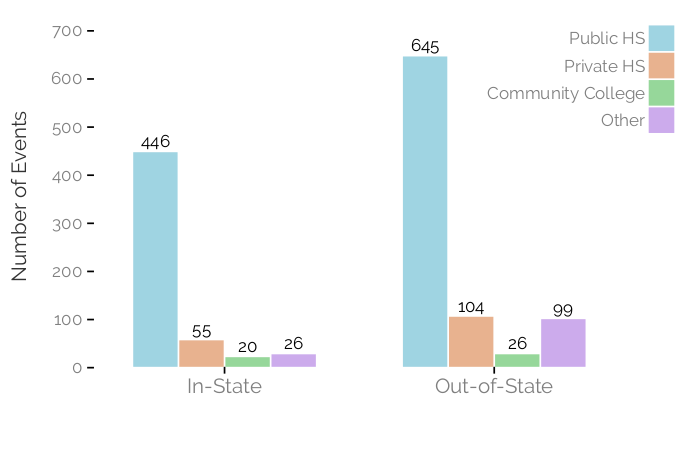
\includegraphics[width=0.45\textwidth, cfbox=LightGray 1pt]{images/#1/visit_count}\hfill
      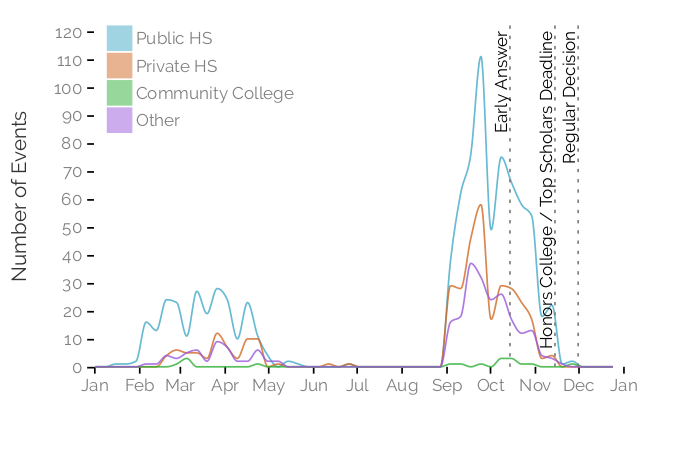
\includegraphics[width=0.45\textwidth, cfbox=LightGray 1pt]{images/#1/timeline}
      
      \smallskip
      
       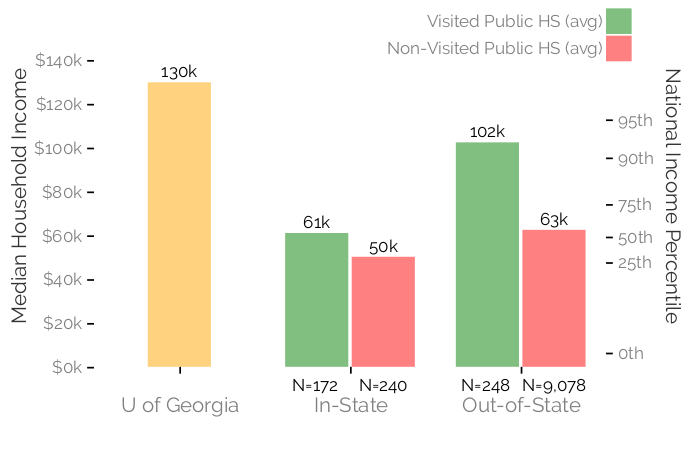
\includegraphics[width=0.45\textwidth, cfbox=LightGray 1pt]{images/#1/median_income}\hfill
       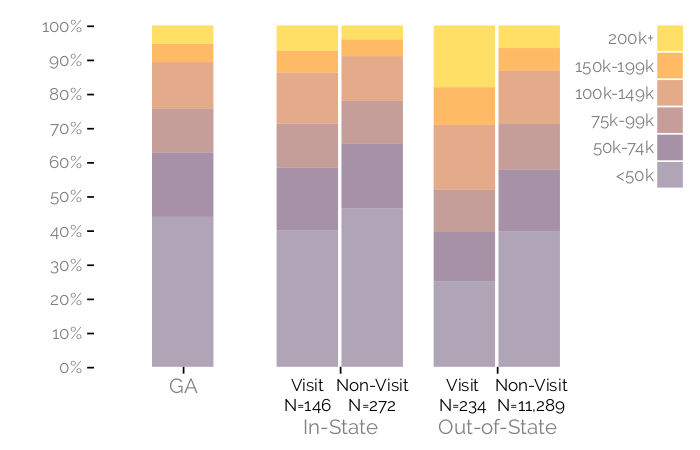
\includegraphics[width=0.45\textwidth, cfbox=LightGray 1pt]{images/#1/income_band}
  \caption{\TradeGothic\selectfont\textcolor{colorFooter}{\uppercase{#2}}}
  \label{fig:#3}
  \vspace{0.45cm}
\end{figure}
}

\newcommand{\addFigureCompare}[2] {

\begin{figure}[!h]
  \vspace{0.45cm}
  \hspace{-1.6in}
  \color{Gray}\hdashrule{1.5\textwidth}{1pt}{1pt}\vspace{0.5cm}
  
  \centering
  
      \makebox[0.79\paperwidth][c]{\hspace{-3cm}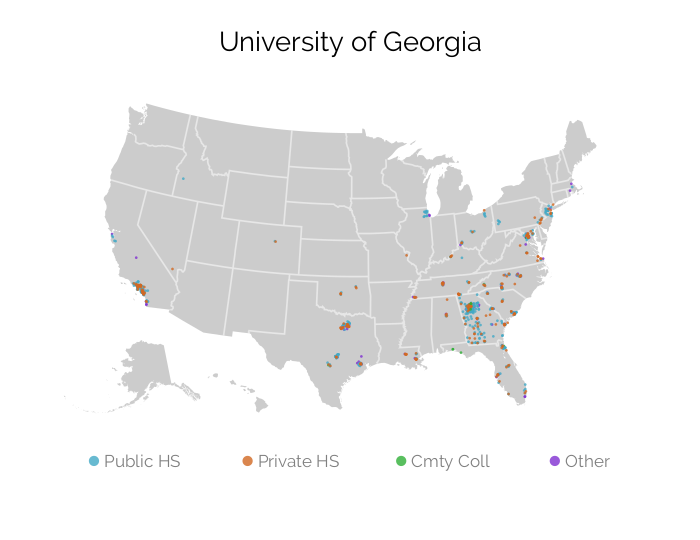
\includegraphics[width=0.2\paperwidth, cfbox=LightGray 1pt]{images/139959/titled_map}\hfill
      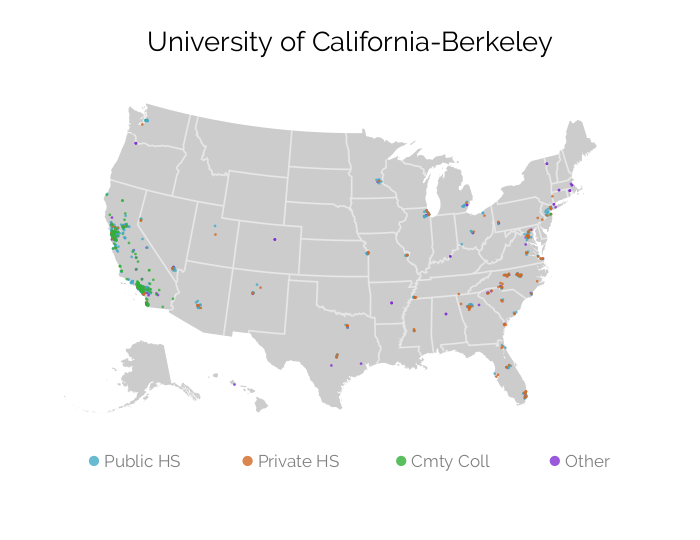
\includegraphics[width=0.2\paperwidth, cfbox=LightGray 1pt]{images/110635/titled_map}\hfill
       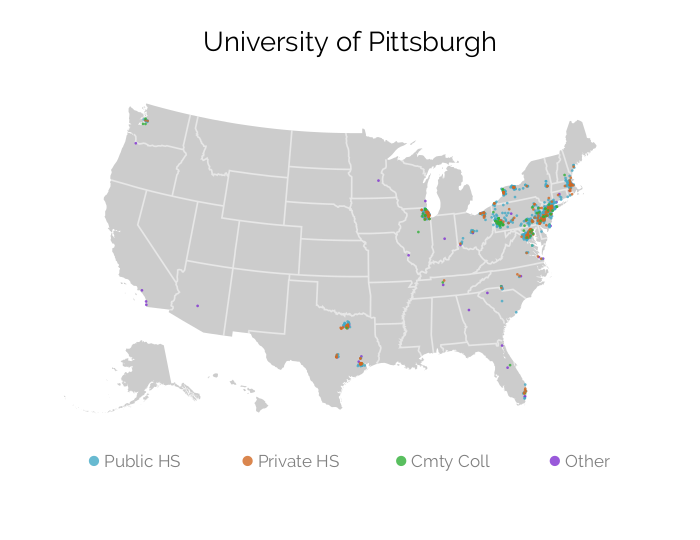
\includegraphics[width=0.2\paperwidth, cfbox=LightGray 1pt]{images/215293/titled_map}\hfill
       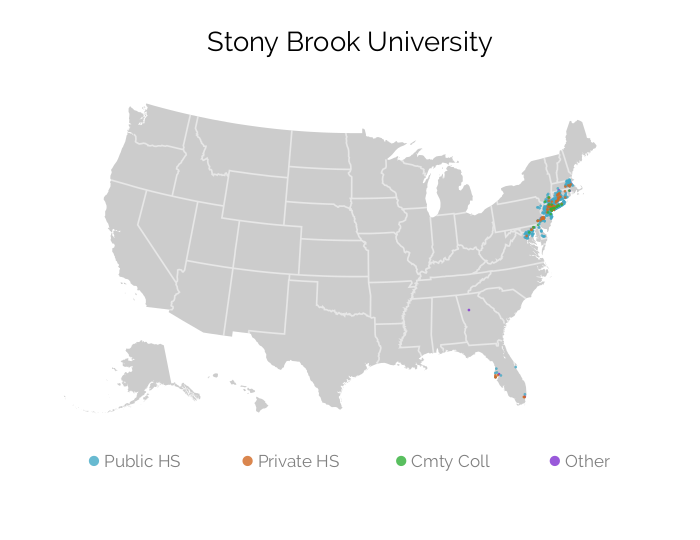
\includegraphics[width=0.2\paperwidth, cfbox=LightGray 1pt]{images/196097/titled_map}}
  \caption{\TradeGothic\selectfont\textcolor{colorFooter}{\uppercase{#1}}}
  
  \label{fig:#2}
  
  \makebox[0.79\paperwidth][c]{\hdashrule{1.5\paperwidth}{1pt}{1pt}}
  
    
\end{figure}

\vspace{0.45cm}

}
    
\usepackage{mdframed}
    
\newenvironment{odd-env}{  % Light-gray Background, Half Page
	\vspace{0.5cm}
	% \begin{minipage}[c]{\textwidth}
	\begin{mdframed}[backgroundcolor=LightBlue, linecolor=LightBlue, userdefinedwidth=8in, leftmargin=0cm, innerleftmargin=1cm, innerrightmargin=6cm, innertopmargin=0.5cm, innerbottommargin=1cm]
	\color{white}
}
{
	\end{mdframed}
	% \end{minipage}
	\vspace{0.5cm}
}

\newenvironment{bottom-env}{  % Light-gray Background, Half Page
	\begin{figure*}[b]
	\vspace{0.2cm}
	\begin{minipage}[b][0.5\textheight][t]{\textwidth}
	\begin{mdframed}[backgroundcolor=LightBlue, linecolor=White, userdefinedwidth=8in, leftmargin=-2cm, innerleftmargin=2cm, innerrightmargin=2cm, innertopmargin=1cm]
}
{
	\vspace{\textheight}
	\end{mdframed}
	\end{minipage}
	\end{figure*}
}


% Links + Lists ~~~~

\PassOptionsToPackage{hyphens}{url}\usepackage[colorlinks=true, linkcolor=cyan, urlcolor=blue, citecolor=blue]{hyperref}
\newcommand{\superscript}[1]{$^{#1}$}

\usepackage[super,numbers]{natbib}

\makeatletter
\renewcommand\@biblabel[1]{\superscript{#1}}
\makeatother

\renewcommand{\refname}{\vspace{-0.65cm}}


%\usepackage{pgffor}
%\usepackage{enumitem}
%\newcommand{\superscript}[1]{$^{#1}$}
%
%\usepackage[super,numbers]{natbib}
%
%\makeatletter
%\renewcommand\@biblabel[1]{\superscript{#1}}
%\makeatother
%
%\renewcommand{\refname}{\vspace{-0.65cm}}
\usepackage{enumitem}
\setlist{nosep, itemsep=0pt, parsep=0pt, before={\TradeGothic\large\color{Gray}}}

\renewcommand{\labelitemi}{\color{colorTitle}$\triangleright$}
\renewcommand{\labelitemii}{\color{Periwinkle}$\cdot$}
\renewcommand\labelitemiii{$\circ$}

% Page Layout ~~~~

\usepackage{geometry}

\geometry{
	letterpaper,
	top=1.75in,
	bottom=1.75in,
	inner=1in,
	outer=1.5in,
	headsep=1in,
	headheight=0.5in,
	footskip=1.2in,
%	showframe
}

%\usepackage{etoolbox}
%\AfterEndEnvironment{figure-env}{\restoregeometry\twocolumn\pagecolor{white}}
%\AfterEndEnvironment{table-env}{\restoregeometry\twocolumn\pagecolor{white}}


% Headers + Footers ~~~~

\usepackage{fancyhdr}
\pagestyle{fancy}

\renewcommand{\sectionmark}[1]{\markboth{#1}{}}
\usepackage{fourier-orns}

\fancyhead{} % clear all header fields
%\fancyhead[RO,LE]{\TradeGothic\fontsize{9pt}{10.8pt}\selectfont\uppercase{\textbf{Oh, The Places They'll Go}}}
\fancyfoot{} % clear all footer fields
\fancyfoot[LE]{\thepage \hspace{0.4cm} \TradeGothic\selectfont\textcolor{colorTitle}{\uppercase{OH, THE PLACES THEY'LL GO}}}
\fancyfoot[RO]{\TradeGothic\selectfont\textcolor{colorFooter}{\leftmark} \hspace{0.4cm} \thepage}
\renewcommand{\headrulewidth}{0pt}
%\renewcommand{\footrulewidth}{0.4pt}

%\renewcommand{\headrulewidth}{0.5pt} 
%\lhead{\TradeGothic\fontsize{9pt}{10.8pt}\selectfont\uppercase{\textbf{Oh, The Places They'll Go}} \vspace{0.3cm}}
%\chead{}
%\rhead{\TradeGothic\fontsize{9pt}{10.8pt}\selectfont\uppercase{Jack Kent Cooke Foundation} \vspace{0.3cm}}
%
%\renewcommand{\footrulewidth}{0.5pt}
%\lfoot{}
%\cfoot{\vspace{0.7cm} \thepage}
%\rfoot{}
%
%\fancypagestyle{coverpage}{  % No Header, No Footer
%    \fancyhf{} 
%    \renewcommand{\headrulewidth}{0pt} 
%    \renewcommand{\footrulewidth}{0pt}
%}

\fancypagestyle{tablepage}{  % No Header, Regular Footer
    \fancyhead{}
    \fancyfoot{}
    \renewcommand\headrule{\hrulefill
\raisebox{-2.1pt}[10pt][10pt]{\quad\decofourleft\decotwo\decofourright\quad}\hrulefill}
}

%\fancypagestyle{figurepage}{  % No Header, White Footer
%    \fancyhead{} 
%    \renewcommand{\headrulewidth}{0pt} 
%    \cfoot{\vspace{0cm} \textcolor{white} \thepage}
%    \renewcommand{\footrule}{\color{white}\hrule width\headwidth \vspace{0.75cm}}
%}


% Page Formats ~~~~

\newenvironment{quote-block}{
	\begin{quote}
	\TradeGothic\selectfont
	\color{colorSection}
	\begin{large}
}
{
	\end{large}
	\end{quote}
}

\newenvironment{table-env}{  % Lightgray Background
	\clearpage
    	\thispagestyle{tablepage}
    	\pagecolor{Gray}
    	\newcommand{?}{?}
	geometry{top=0.75in, bottom=0.75in, left=0.75in, right=0.75in, footskip=0in}
	\onecolumn

}
{ 
    	\clearpage
}

%\newenvironment{figure-env}{  % Gray Background, White Text
%	\clearpage
%	\thispagestyle{figurepage}
%    	\pagecolor{Gray}
%   	\color{white}
%    	\newgeometry{top=0.75in, bottom=0.8in, left=0.75in, right=0.75in, footskip=0in}
%	\onecolumn
%}
%{
%	\clearpage
%}
%
%\newenvironment{bottom-table-env}{  % Gray Background, Half Page
%	\begin{figure*}[b]
%%	\vspace{0.2cm}
%	\begin{minipage}[b][0.5\textheight][t]{\textwidth}
%	\begin{mdframed}[backgroundcolor=Gray, linecolor=Gray, userdefinedwidth=8in, leftmargin=-2cm, innerleftmargin=2cm, innerrightmargin=2cm, innertopmargin=1cm]
%	\Avenir\fontsize{9pt}{12pt}\selectfont
%}
%{
%	\vspace{\textheight}
%	\end{mdframed}
%	\end{minipage}
%	\end{figure*}
%}
